\documentclass[11pt,a4paper]{article}
\usepackage[margin=1in]{geometry}
\usepackage{graphicx}
\usepackage{float}
\usepackage[hidelinks]{hyperref}
\setlength{\parskip}{0.6em}
\setlength{\parindent}{0pt}
\title{A granular expenditure-side decomposition of Portuguese GDP growth}
\author{Diogo Ribeiro}
\date{}
\begin{document}
\maketitle
This report documents the measurement choices, the system model, and the analytical extensions behind the Portuguese GDP contribution decomposition, and states what each layer does and does not support. It is generated directly from the pipeline artifacts; every number below is read from a table in \texttt{output/} and every figure it shows was produced in the same run. The estimation is carried out in Python with statsmodels \cite{statsmodels}.
\section{Data and measurement}
The raw material is Eurostat's quarterly national accounts for Portugal, \texttt{namq\_10\_gdp}, obtained through DBnomics. Two unit variants are pulled for the same expenditure items: chain-linked volumes with reference year 2020 (\texttt{CLV20\_MEUR}), which carry the real quarter-on-quarter dynamics over 119 quarters of usable observations, and current prices (\texttt{CP\_MEUR}), which supply the nominal weights used to turn volume changes into contributions. Both are seasonally and calendar adjusted (SCA); working with the adjusted series keeps the quarter-on-quarter growth rates free of the deterministic seasonal pattern that would otherwise dominate the contributions and forces any seasonality in the later state-space models to be treated as a modelling option rather than a nuisance to be differenced away.
Two measurement facts shape everything downstream. The first is a vintage issue: some releases publish changes in inventories (P52) and acquisitions of valuables (P53) only as a combined \texttt{P52\_P53} series, so the code resolves whichever set is present and labels the combined item accordingly rather than silently dropping inventories. The second is chain-linking non-additivity. Chain-linked volumes are not additive away from the reference year, so the component volumes do not sum to the GDP volume and the naive contribution residual against GDP growth is non-zero. The convention-comparison table quantifies it: over the sample the exact annual-overlap residual averages 0.0071 pp with a maximum absolute value of 1.901 pp, while the raw naive approximation residual averages -0.0081 pp with a maximum absolute value of 1.409 pp. After proportional reallocation the identity closes to a maximum absolute residual of 1.8e-15 pp, which is the number the system model relies on.
The division of labour between the two unit variants is worth making explicit because it is the source of most confusion in contribution accounting. Volumes answer 'how much more was produced or spent', stripping out price change, and so they carry the growth signal; current prices answer 'how large was each component in money terms', and so they carry the weights that convert a component's own growth into its share of headline growth. Using volume shares as weights would double-count relative price movements, which is precisely the trap the exact method in the next section avoids. The reference year matters here too: at 2020 prices the volume aggregates are additive in and around 2020 and drift apart the further a quarter sits from that year, so the non-additivity is not a data error to be cleaned but a structural feature of chain-linking that the accounting has to confront head-on.
\begin{figure}[H]\centering
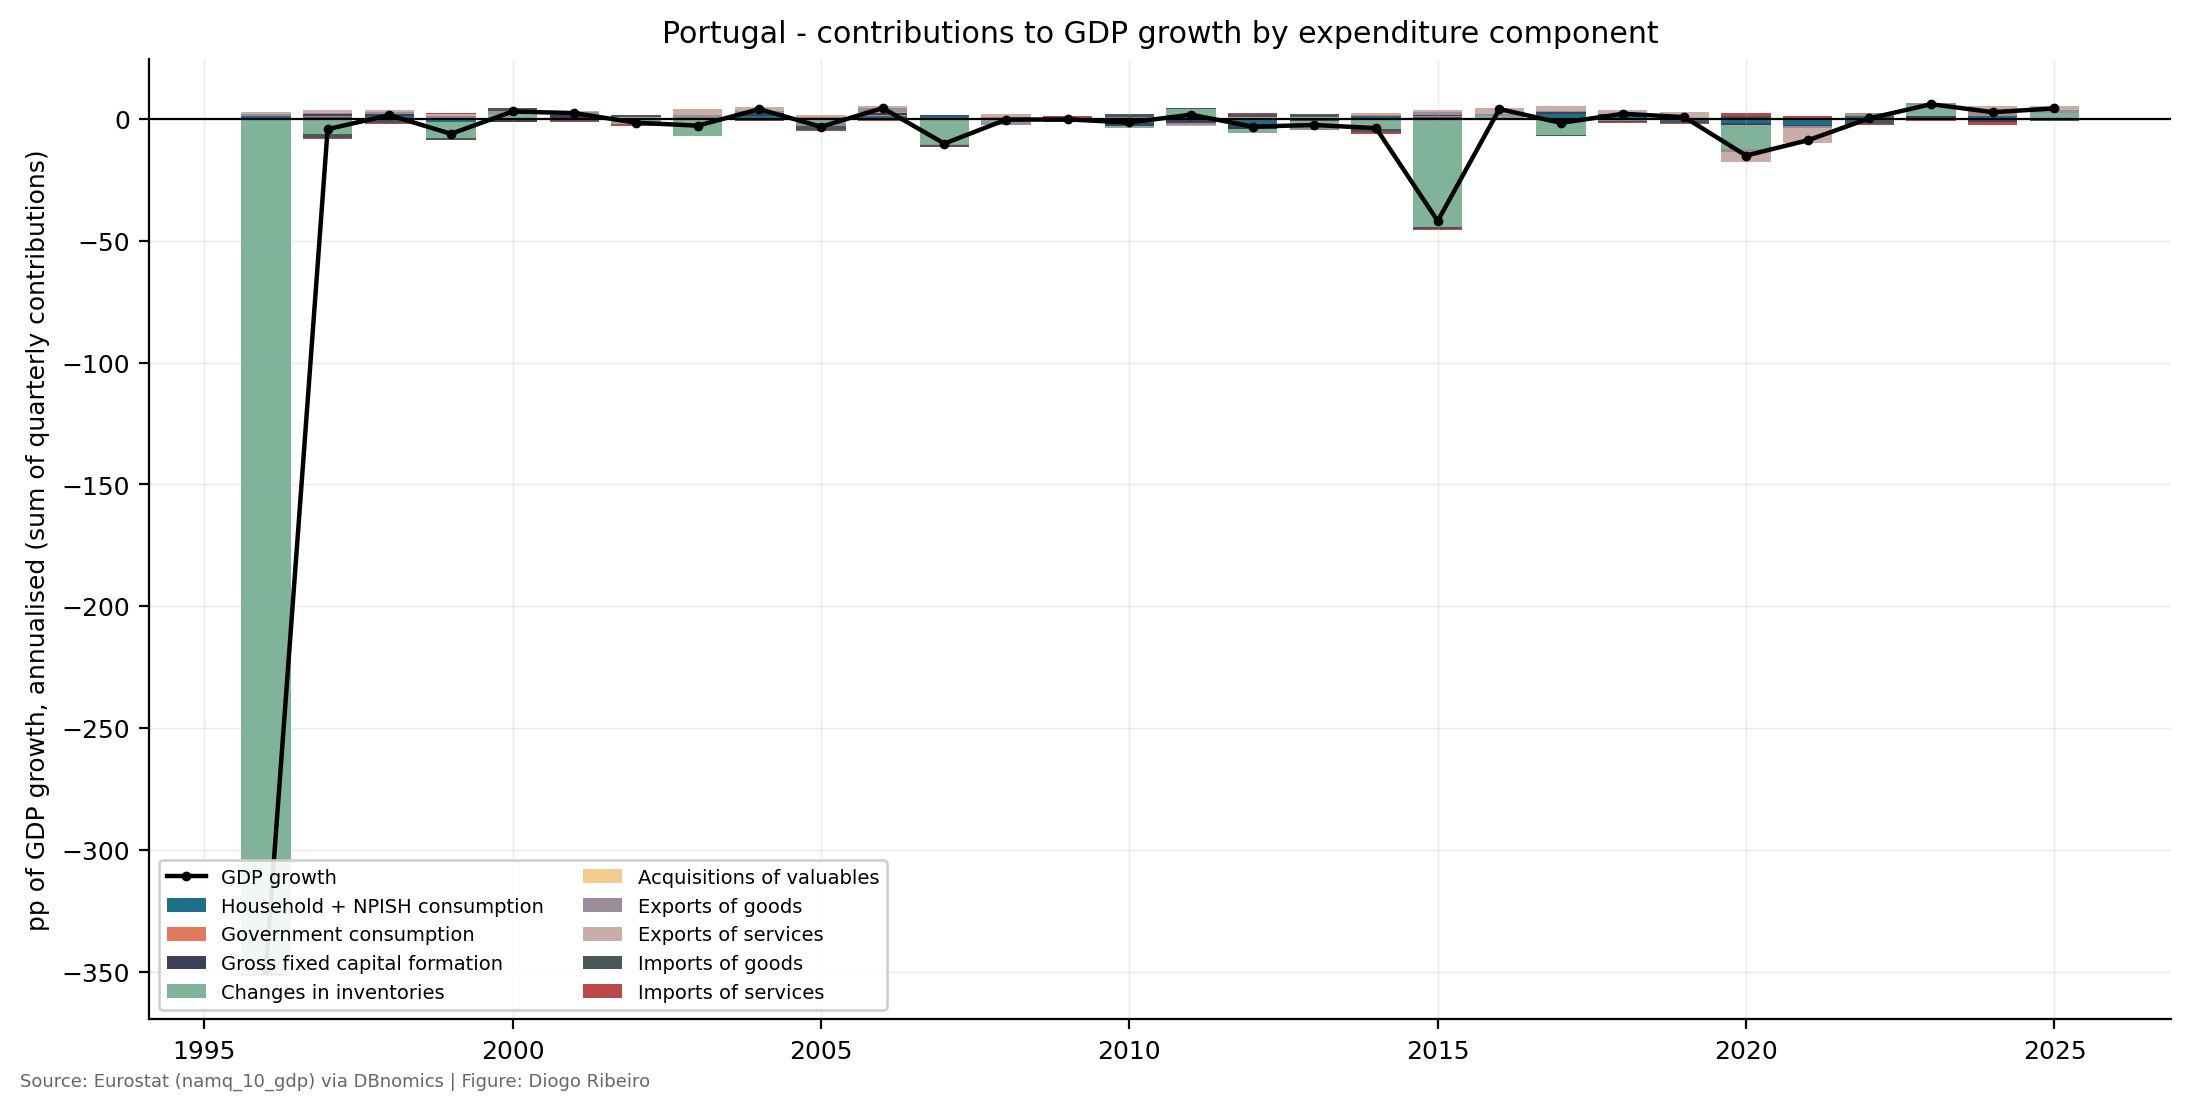
\includegraphics[width=\linewidth]{../output/contributions_stacked.png}
\caption{Contributions to Portuguese GDP growth by expenditure component, annualised}
\end{figure}


\section{Contribution methodology}
The default contributions use the annual-overlap exact formula: each component's quarter-on-quarter volume ratio is weighted by its share of nominal GDP in the previous calendar year, \texttt{contrib = sign x s\_prev x (X\_t / X\_prev - 1) x 100}, with the nominal shares taken from annual sums of the current-price frame. This is the additive decomposition consistent with a chain-linked Laspeyres aggregate \cite{eurostatqna}, in which the aggregate within a linking year is a fixed-previous-year-price index and previous-year nominal shares are therefore the correct weights. The naive alternative, differencing the volume level and dividing by lagged GDP, is retained only as a robustness check because it treats volume levels measured in reference-year prices as if they were additive across components. The two conventions leave maximum absolute residuals of 1.409 pp (naive) and 1.901 pp (exact). The exact method is preferred not because it always leaves the smaller residual --- the ratio form can amplify quarters in which a small component's volume swings sharply, and on this sample its maximum residual is in fact the larger of the two --- but because its previous-year nominal weights are the correct ones for a chain-linked aggregate, whereas the naive shortcut's implied reference-year-price weights have no such justification. Whichever convention is chosen, the small remaining residual is reallocated proportionally to the absolute size of each contribution so that the adding-up identity the system model needs holds by construction rather than by assumption.
The intuition for the previous-year weights is that a chain-linked volume index is built by stitching together annual links, each of which is a fixed-price index using the prior year's prices. Within a link, then, a component's marginal contribution to the aggregate is its own volume change scaled by how large it was, in money, the year before --- exactly the previous-year nominal share. The naive difference-over-lagged-GDP shortcut ignores this and implicitly reweights components by their reference-year price levels, which is why its residual has a systematic component that grows with distance from the reference year, a bias the exact method does not share (its residual is near-zero on average and driven by ratio noise rather than reference-year drift). Reporting both conventions is not indecision: it lets a reader see the size of the convention's footprint on any single quarter before deciding whether it matters for the question at hand.
\section{The system model}
Each of the 7 component contribution series is regressed on a common design: an intercept, a linear trend expressed in decades so the coefficient reads as pp of quarterly growth per decade, and two regime dummies for the global financial crisis and troika period (2008Q3--2013Q4) and the pandemic (2020Q1--2021Q4). Because every equation shares the same regressors, seemingly-unrelated regression collapses to equation-by-equation OLS by Kruskal's theorem \cite{kruskal1968}, and because the dependent variables sum to GDP growth by construction, the component coefficient vectors sum across equations to the GDP-growth equation coefficients exactly. The adding-up property is therefore inherited, not imposed, and is verified numerically at run time: in this run the maximum discrepancy between the summed component coefficients and the GDP coefficients is 7.1e-15. Inference uses Newey-West HAC standard errors \cite{neweywest1987} with four lags, the honest choice for quarterly contributions with serial correlation. The estimated GDP-level trend is -0.034 pp of quarterly growth per decade (HAC p = 0.678). The regime means tell the cyclical story the trend cannot: average quarterly GDP growth is 0.578 pp in normal periods, -0.339 pp through the crisis-and-troika window, and 0.324 pp across the pandemic window, the last of these an average over quarters that include both the 2020 collapse and the rebound.
Allowing the trend to break by regime sharpens the reading. Re-centring the interaction trend at each regime's entry lets the dummy measure the level shift at entry and the interaction the within-regime slope change. A joint Wald test on the HAC covariance of the null that both interaction coefficients are zero gives, for the GDP equation, a statistic of 6.914 (p = 0.032); across the individual component equations 2 of 7 reject the no-break null at the 5\% level. The slope-break tests are descriptive of where the static-slope assumption is least comfortable, and they motivate the state-space layer that lets the slope move every quarter.
Two properties of this design deserve emphasis because they are easy to mis-state. First, the equality of SUR and OLS here is exact, not approximate: it follows from Kruskal's theorem the moment every equation shares an identical regressor matrix, so estimating the system buys nothing over the equation-by-equation regressions except the bookkeeping that keeps the adding-up visible. Second, the cross-equation residual covariance is singular by construction, because the component residuals sum to the GDP-equation residual; this is expected and harmless for a design that never inverts that covariance, and it is reported only for inspection. The HAC lag of four quarters is chosen to span a full year of potential residual autocorrelation in quarterly data without over-smoothing the covariance, and the diagnostics section returns to whether four lags is enough.
\begin{figure}[H]\centering
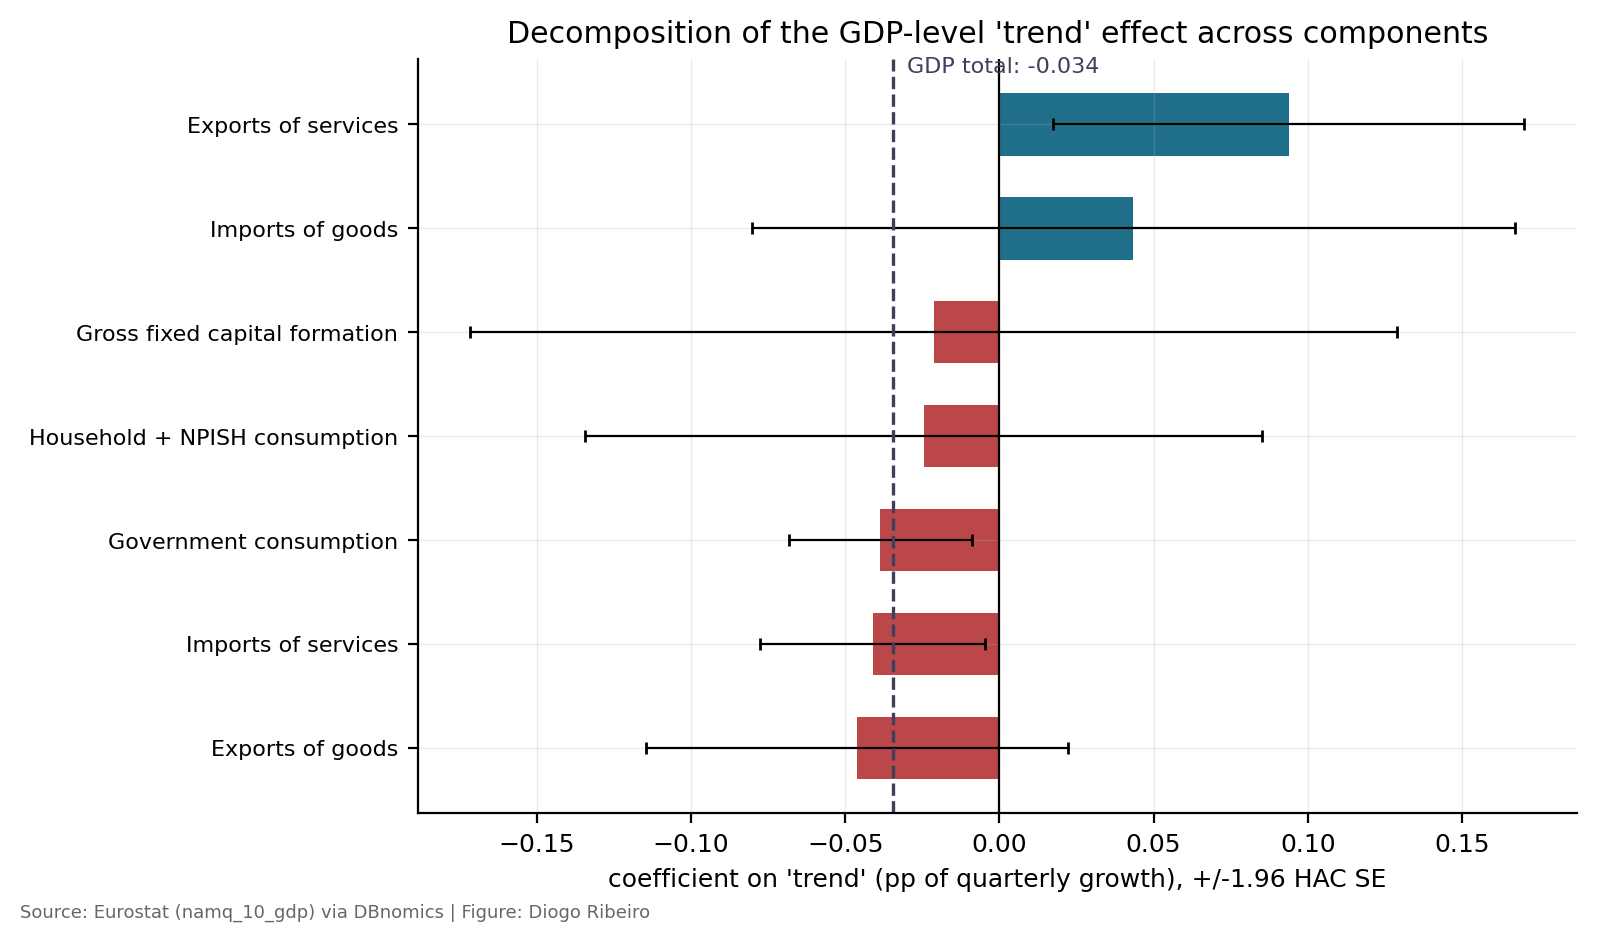
\includegraphics[width=\linewidth]{../output/decomposition_trend.png}
\caption{Decomposition of the GDP-level trend effect across components}
\end{figure}


\begin{figure}[H]\centering
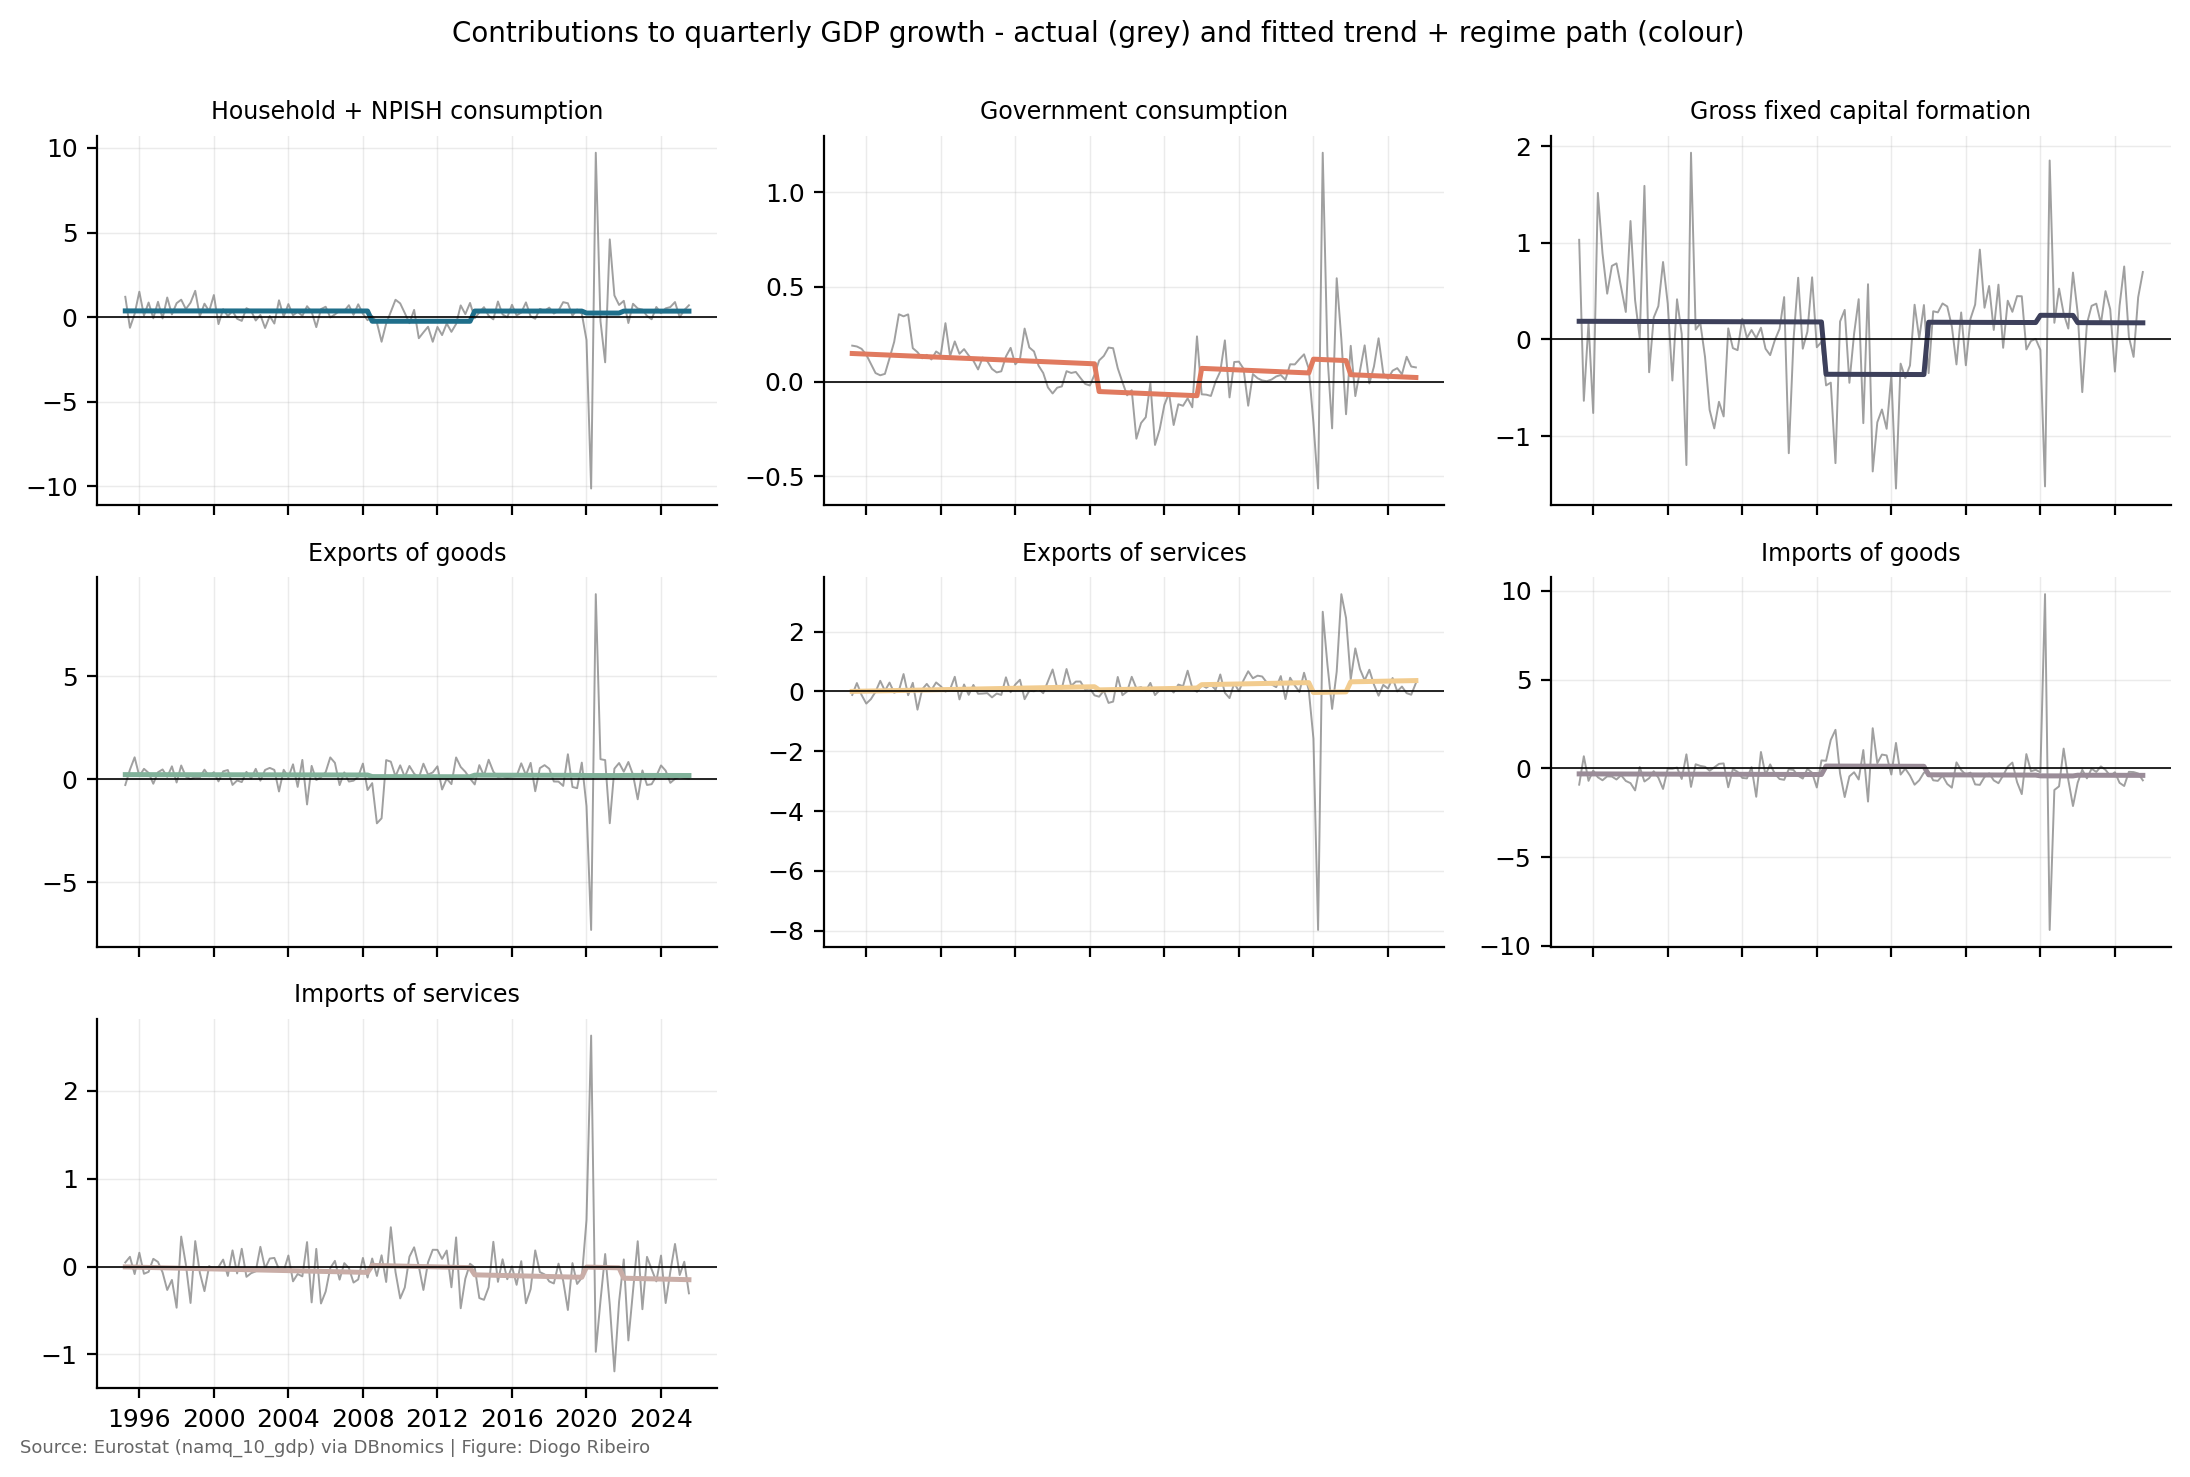
\includegraphics[width=\linewidth]{../output/contributions_small_multiples.png}
\caption{Component contributions with fitted trend-and-regime paths}
\end{figure}


\section{Import-content adjustment}
Gross contributions treat imports as a single negative block, which understates how much of each final-demand component is met from abroad. The import-content adjustment reallocates the combined import contribution across private consumption, public consumption, gross fixed capital formation and exports in proportion to each component's import content, leaving net contributions that still sum to GDP growth. The reading changes from a mechanical exports-minus-imports split to a domestic-versus-external demand split. The essential caveat is that the import-content matrix is an exogenous input, not something estimated here: the default shares are a clearly flagged placeholder derived from Banco de Portugal import-content estimates \cite{bdp2016}, to be replaced with a current input-output vintage, and the domestic-versus-external conclusion is only as good as that matrix.
\begin{figure}[H]\centering
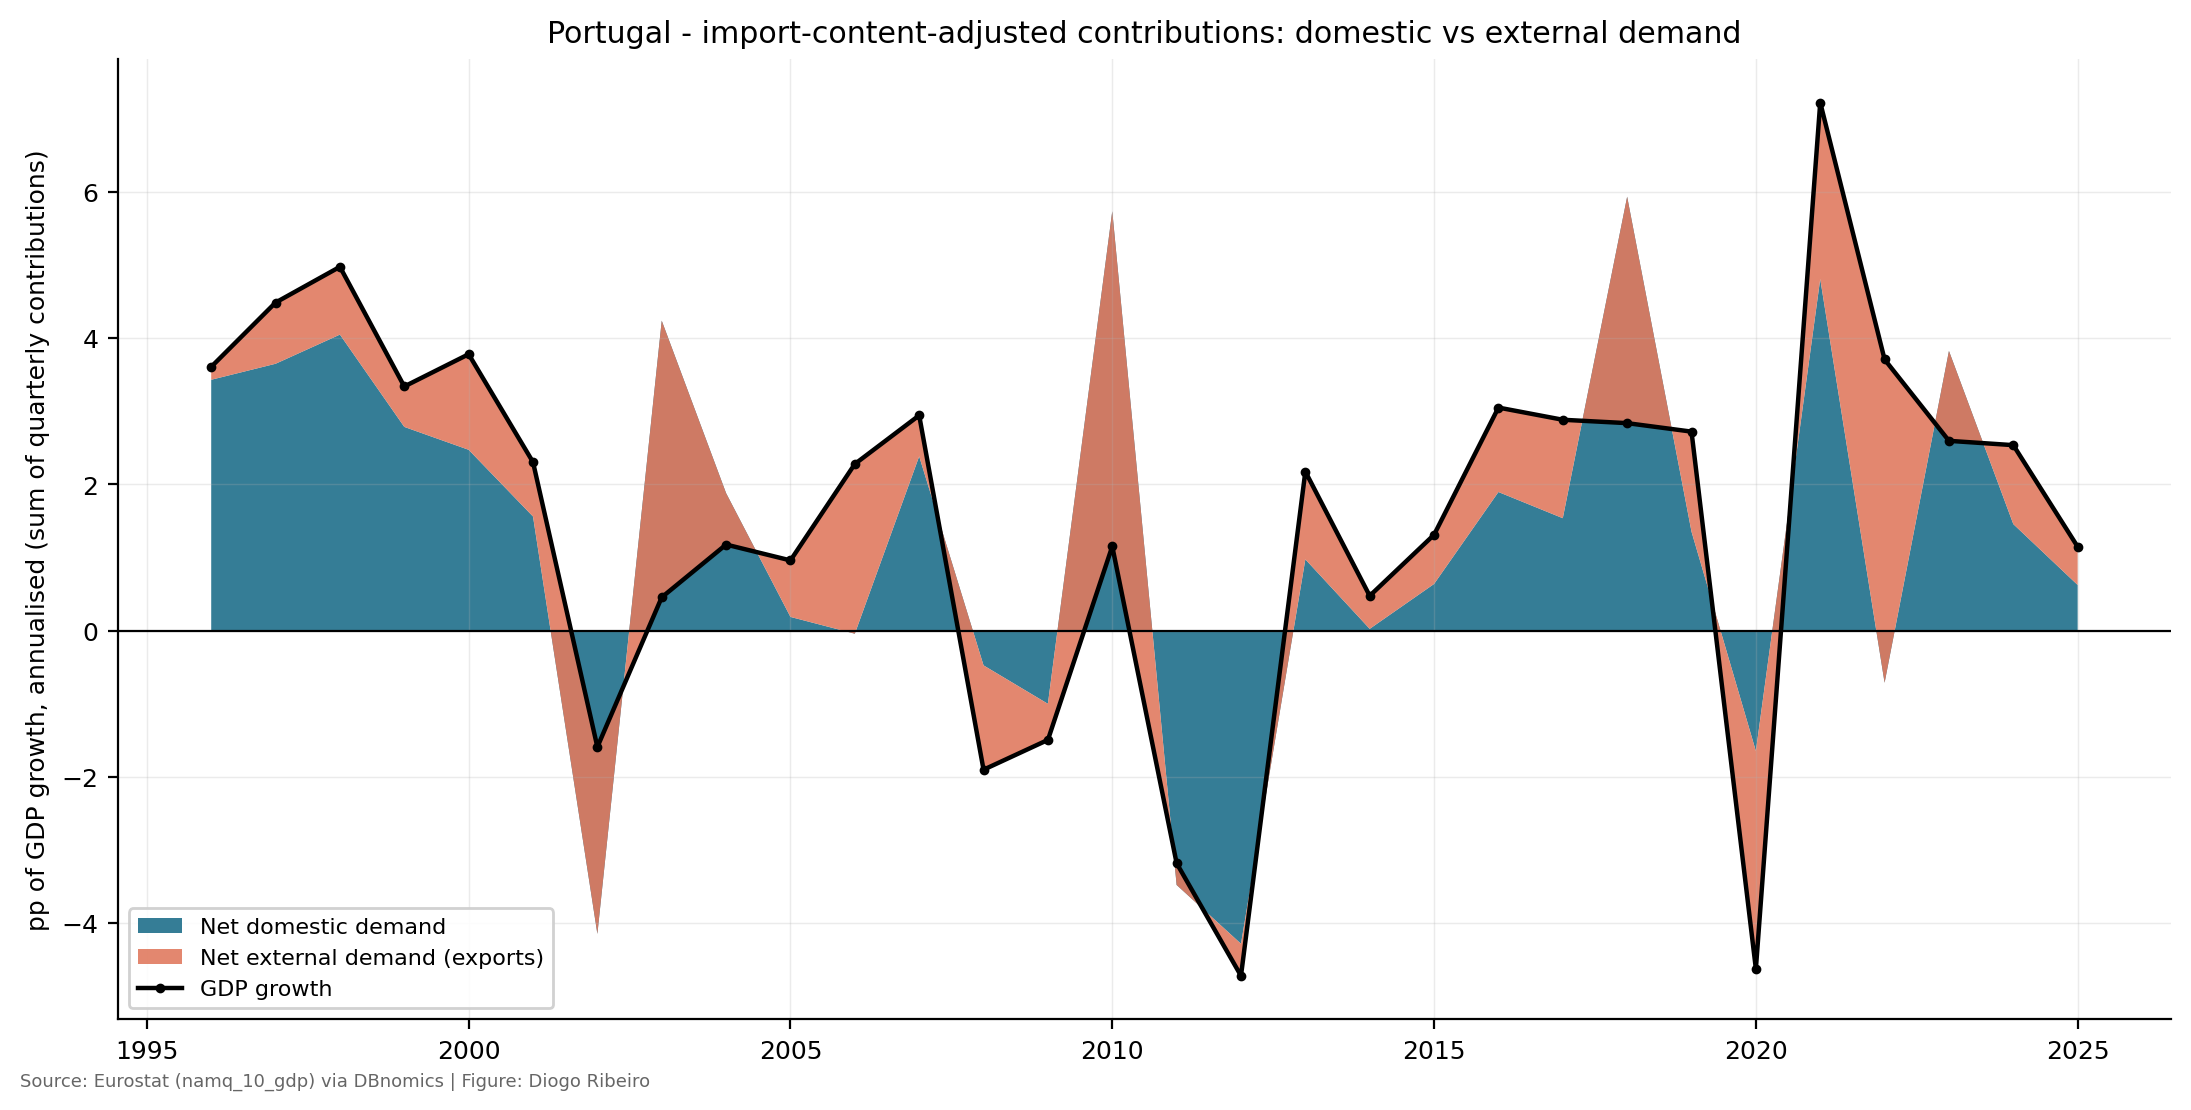
\includegraphics[width=\linewidth]{../output/domestic_vs_external.png}
\caption{Import-content-adjusted contributions: domestic vs external demand}
\end{figure}


\section{Deeper granularity}
Two annual breakdowns add resolution the quarterly ten-component layer cannot carry: gross fixed capital formation by asset type (\texttt{nama\_10\_an6}) and household consumption by COICOP purpose (\texttt{nama\_10\_co3\_p3}). Because these source series are annual, they are used at annual frequency and never interpolated to quarterly. Each year's parent contribution is split across its children in proportion to the children's annual volume changes, with the non-additivity of the child breakdown reallocated proportionally so the split closes onto the parent contribution. The layer is strictly additive to the existing decomposition and leaves the quarterly system untouched; it answers 'which assets' and 'which purposes' without disturbing the 'which components' answer above.
\begin{figure}[H]\centering
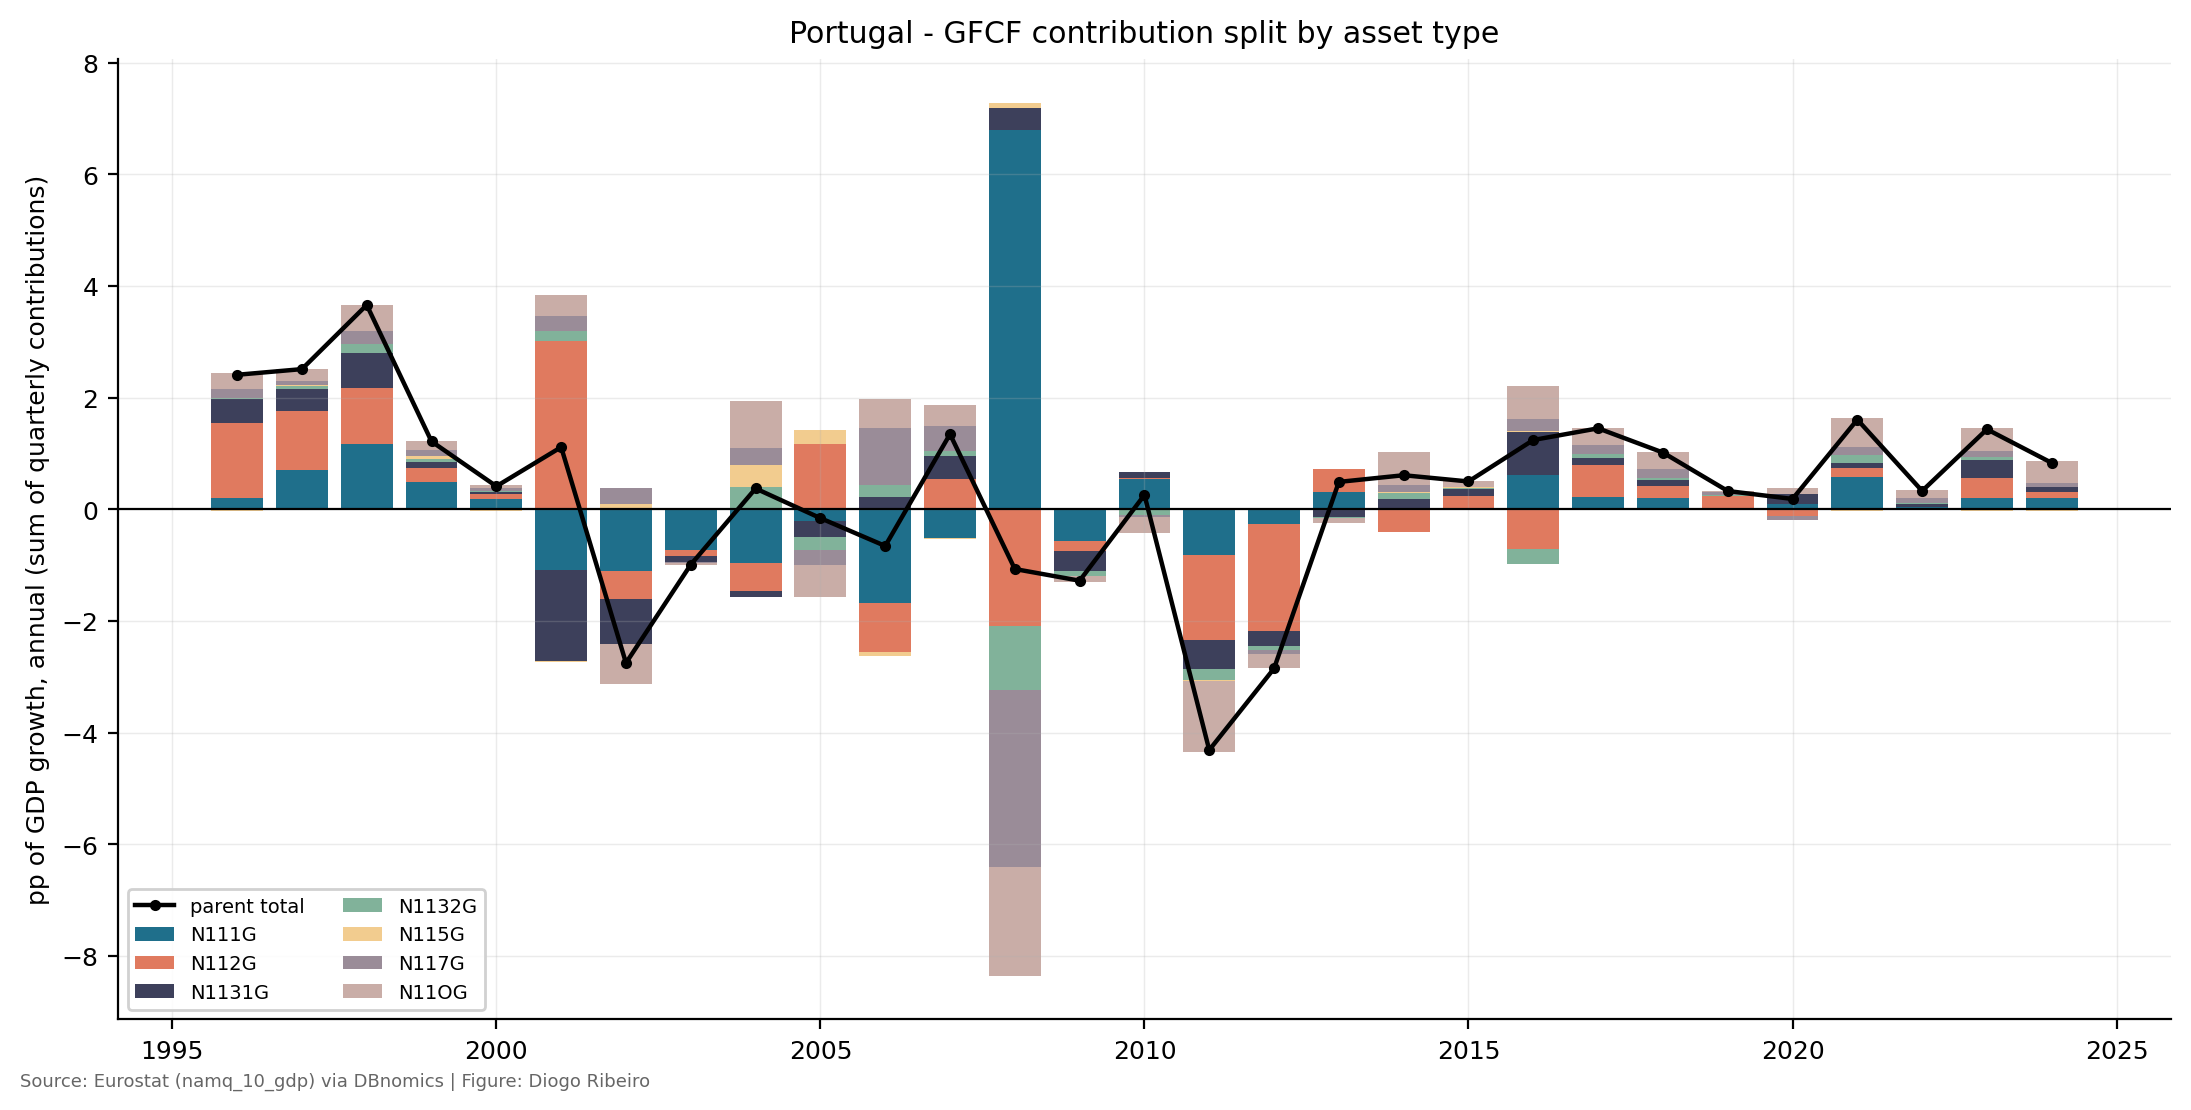
\includegraphics[width=\linewidth]{../output/gfcf_by_asset.png}
\caption{GFCF contribution split by asset type, annual}
\end{figure}


\begin{figure}[H]\centering
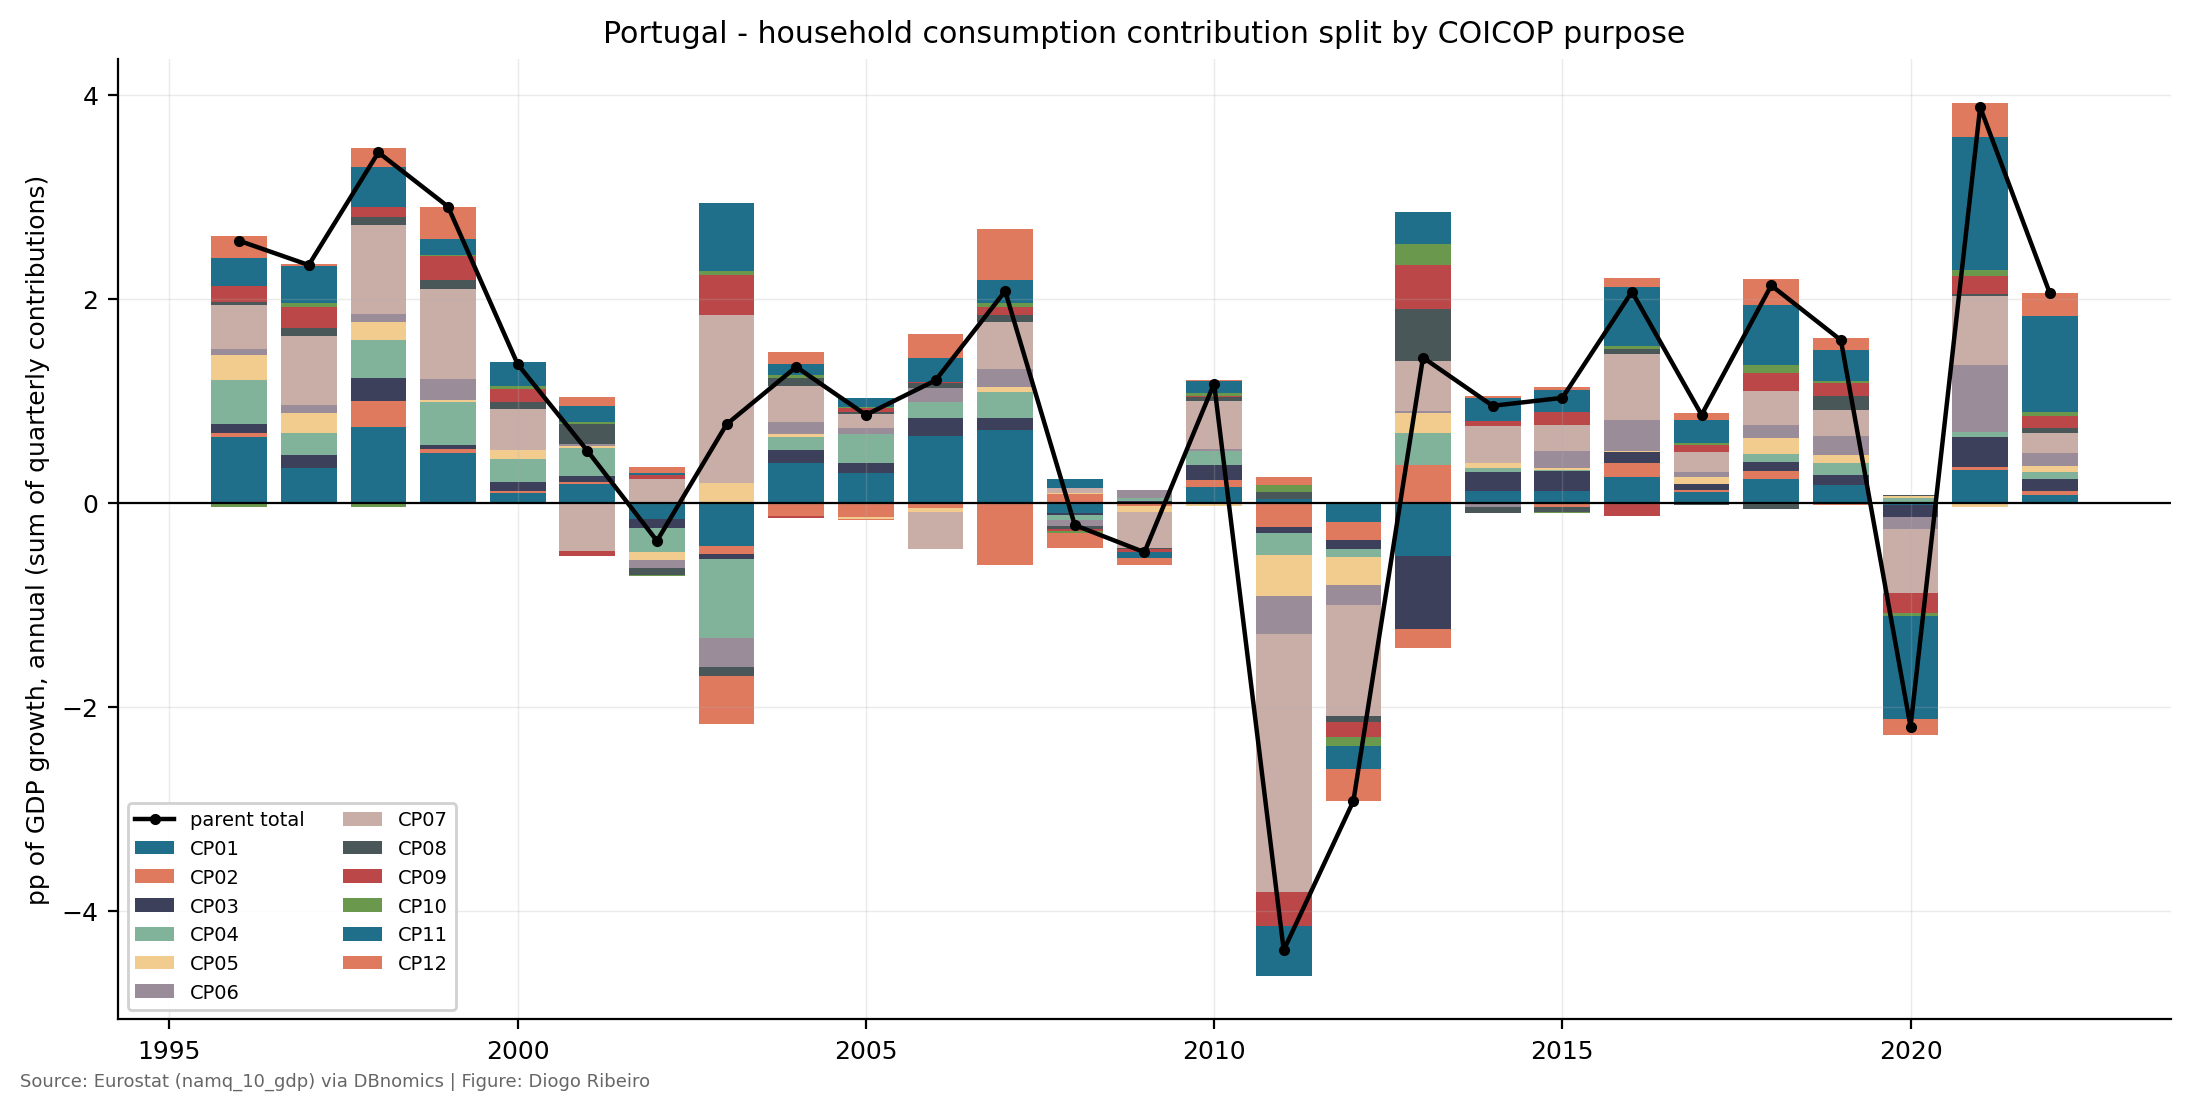
\includegraphics[width=\linewidth]{../output/consumption_by_purpose.png}
\caption{Household consumption contribution split by COICOP purpose, annual}
\end{figure}


\section{Dynamics}
The diagnostics battery tests each equation's residuals for serial correlation (Ljung-Box at lags four and eight \cite{ljungbox1978}), conditional heteroskedasticity (ARCH-LM at lag four \cite{engle1982}), non-normality (Jarque-Bera) and parameter stability (a CUSUM test \cite{plobergerkramer1992}), all reported as p-values. In this run 7 of 8 equations show Ljung-Box p below 0.05 at lag four, which is the diagnostic with teeth. The implication is stated without hedging: HAC standard errors remain valid for inference on the mean parameters even under residual autocorrelation, but a static mean model with autocorrelated residuals is dynamically incomplete as a description of the data. That is a motivation for a time-varying-trend model, not a reason to distrust the reported inference.
\begin{figure}[H]\centering
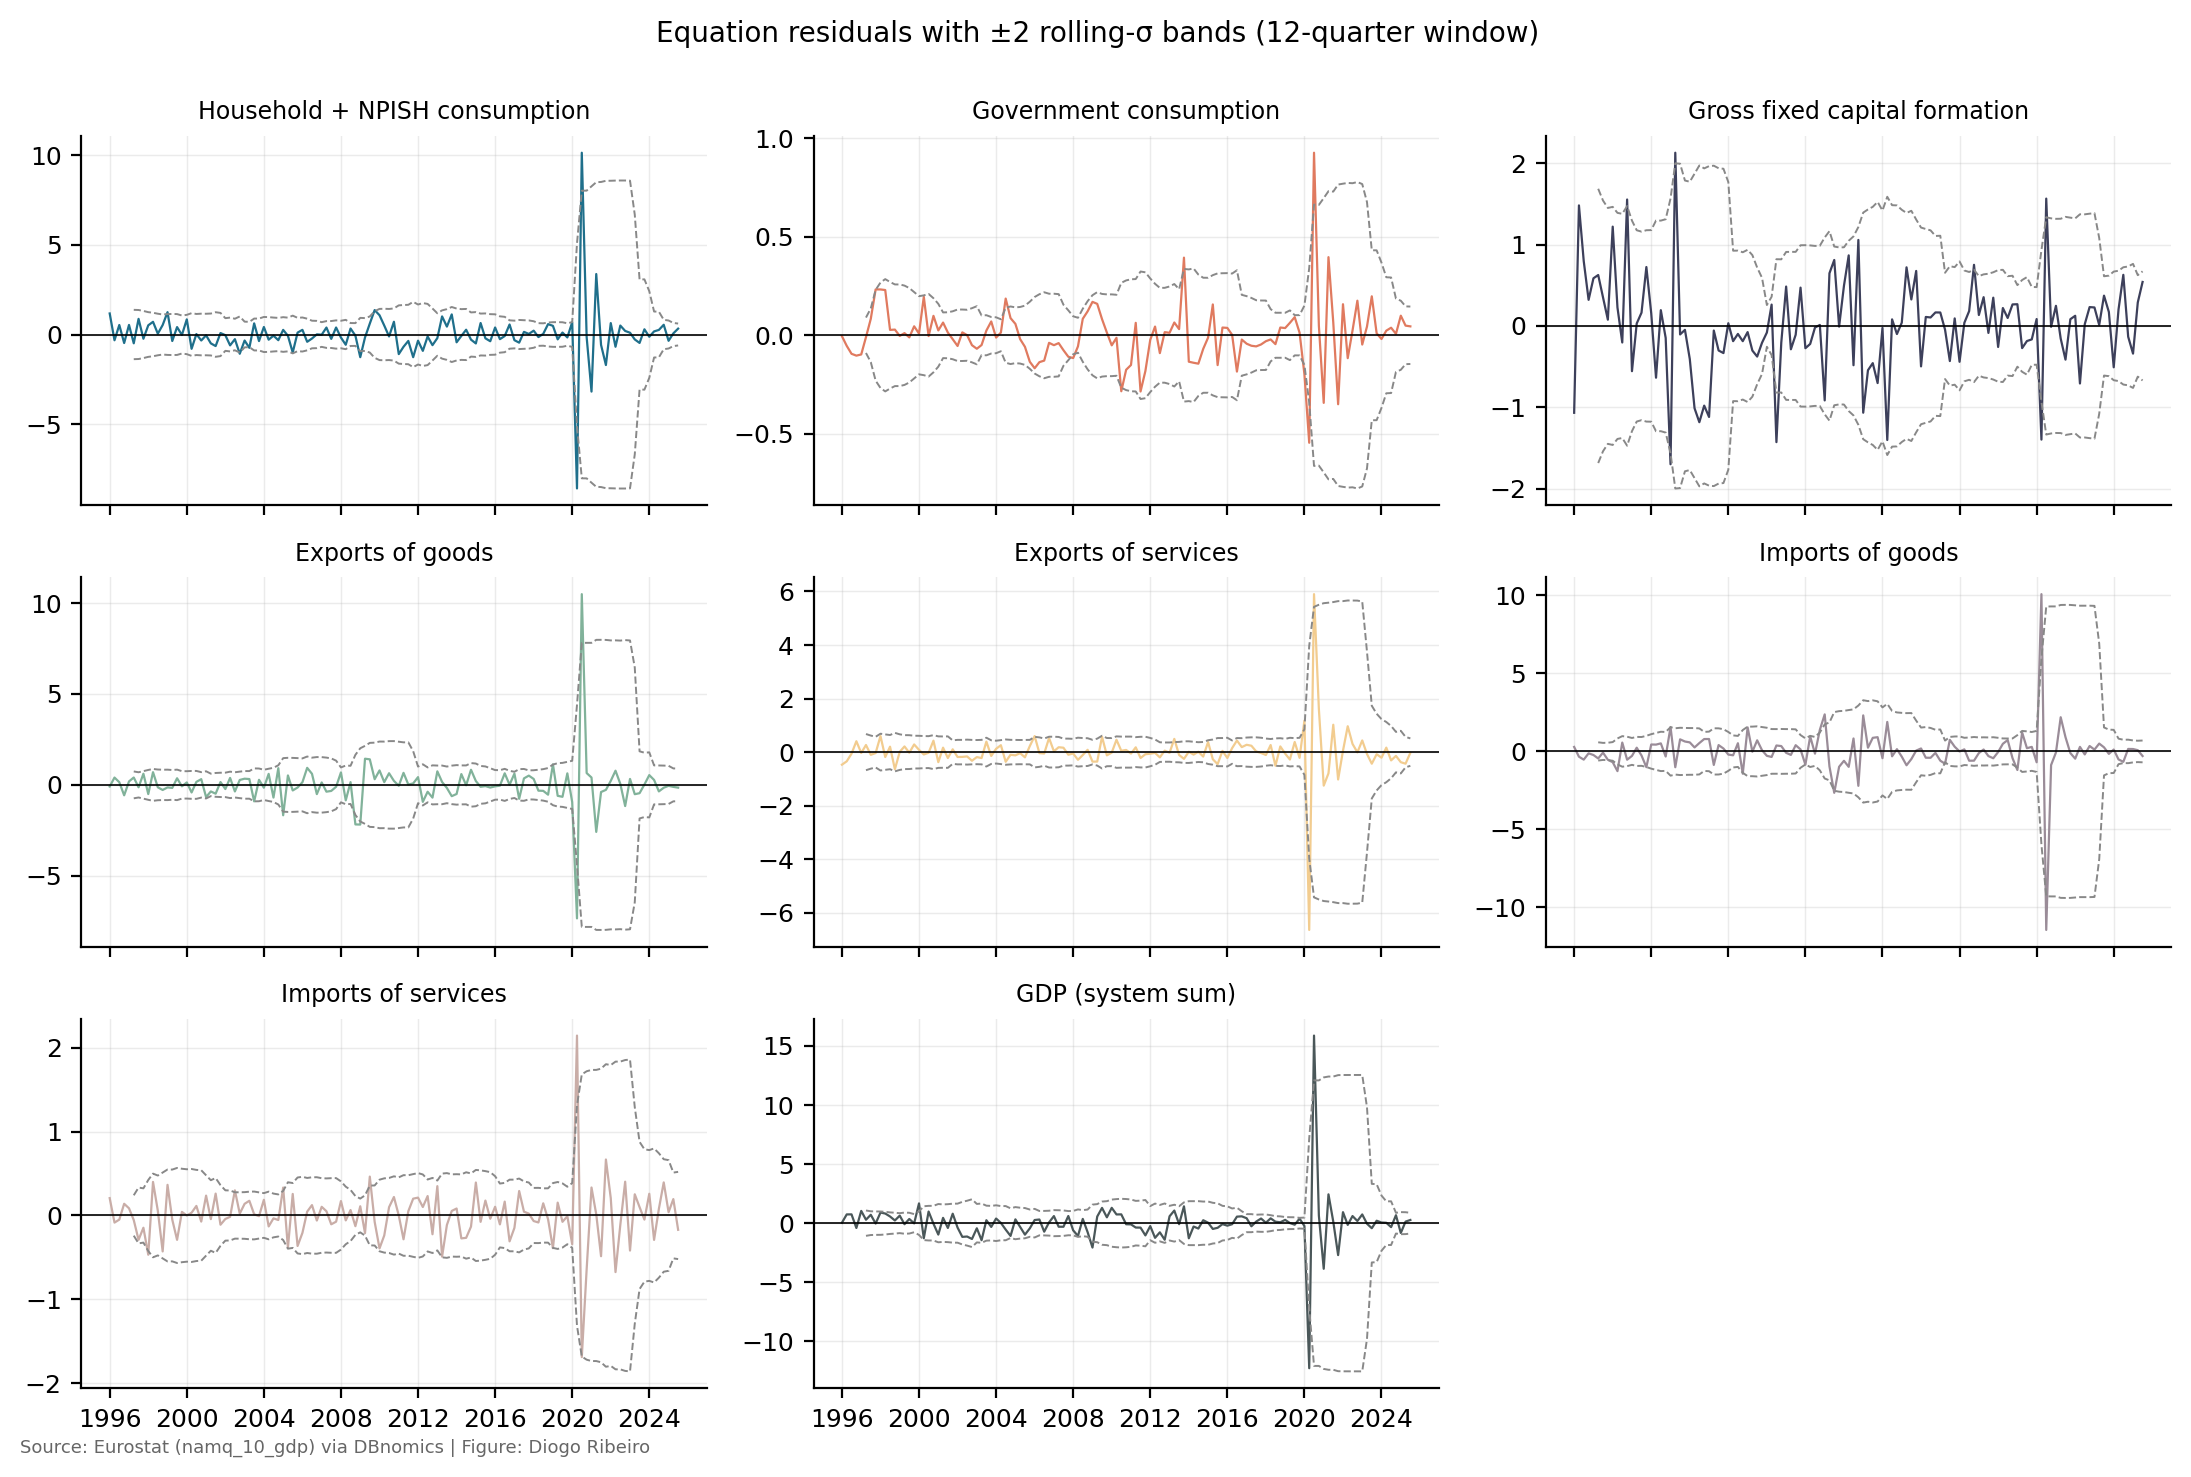
\includegraphics[width=\linewidth]{../output/residual_panel.png}
\caption{Equation residuals with plus/minus two rolling-sigma bands}
\end{figure}


The state-space layer fits a local linear trend to each contribution series and to GDP growth, extracting a smoothed slope path with a 90\% band. The band gives the state-space answer to 'when was the trend real': for GDP growth the 90\% band excludes zero in 0 of 119 quarters. Because the slopes are estimated one series at a time, the adding-up identity is not imposed across the state-space models, and the sum of the smoothed component slopes need not equal the smoothed GDP slope; that gap is reported per quarter as a model-consistency diagnostic and reaches at most 0.004 pp per decade in this run.
A few modelling choices in the state-space layer are worth recording. The level is specified as a local linear trend \cite{harvey1989} --- a stochastic level plus a stochastic slope --- which lets both the position and the direction of a series wander rather than forcing a single straight line through three decades of data. The stochastic seasonal term is off by default because the input is already seasonally adjusted; it is exposed as a flag only so residual seasonality can be probed where it is suspected, not as a routine addition. Estimation is by maximum likelihood, and non-convergence is handled explicitly: a series that fails under the default optimiser is retried under Powell's method and, if it still fails, is logged and skipped rather than silently returning a meaningless path. That the smoothed component slopes do not sum to the smoothed GDP slope is not a bug but the price of estimating each series independently, and the reported per-quarter gap is the receipt for that price.
\begin{figure}[H]\centering
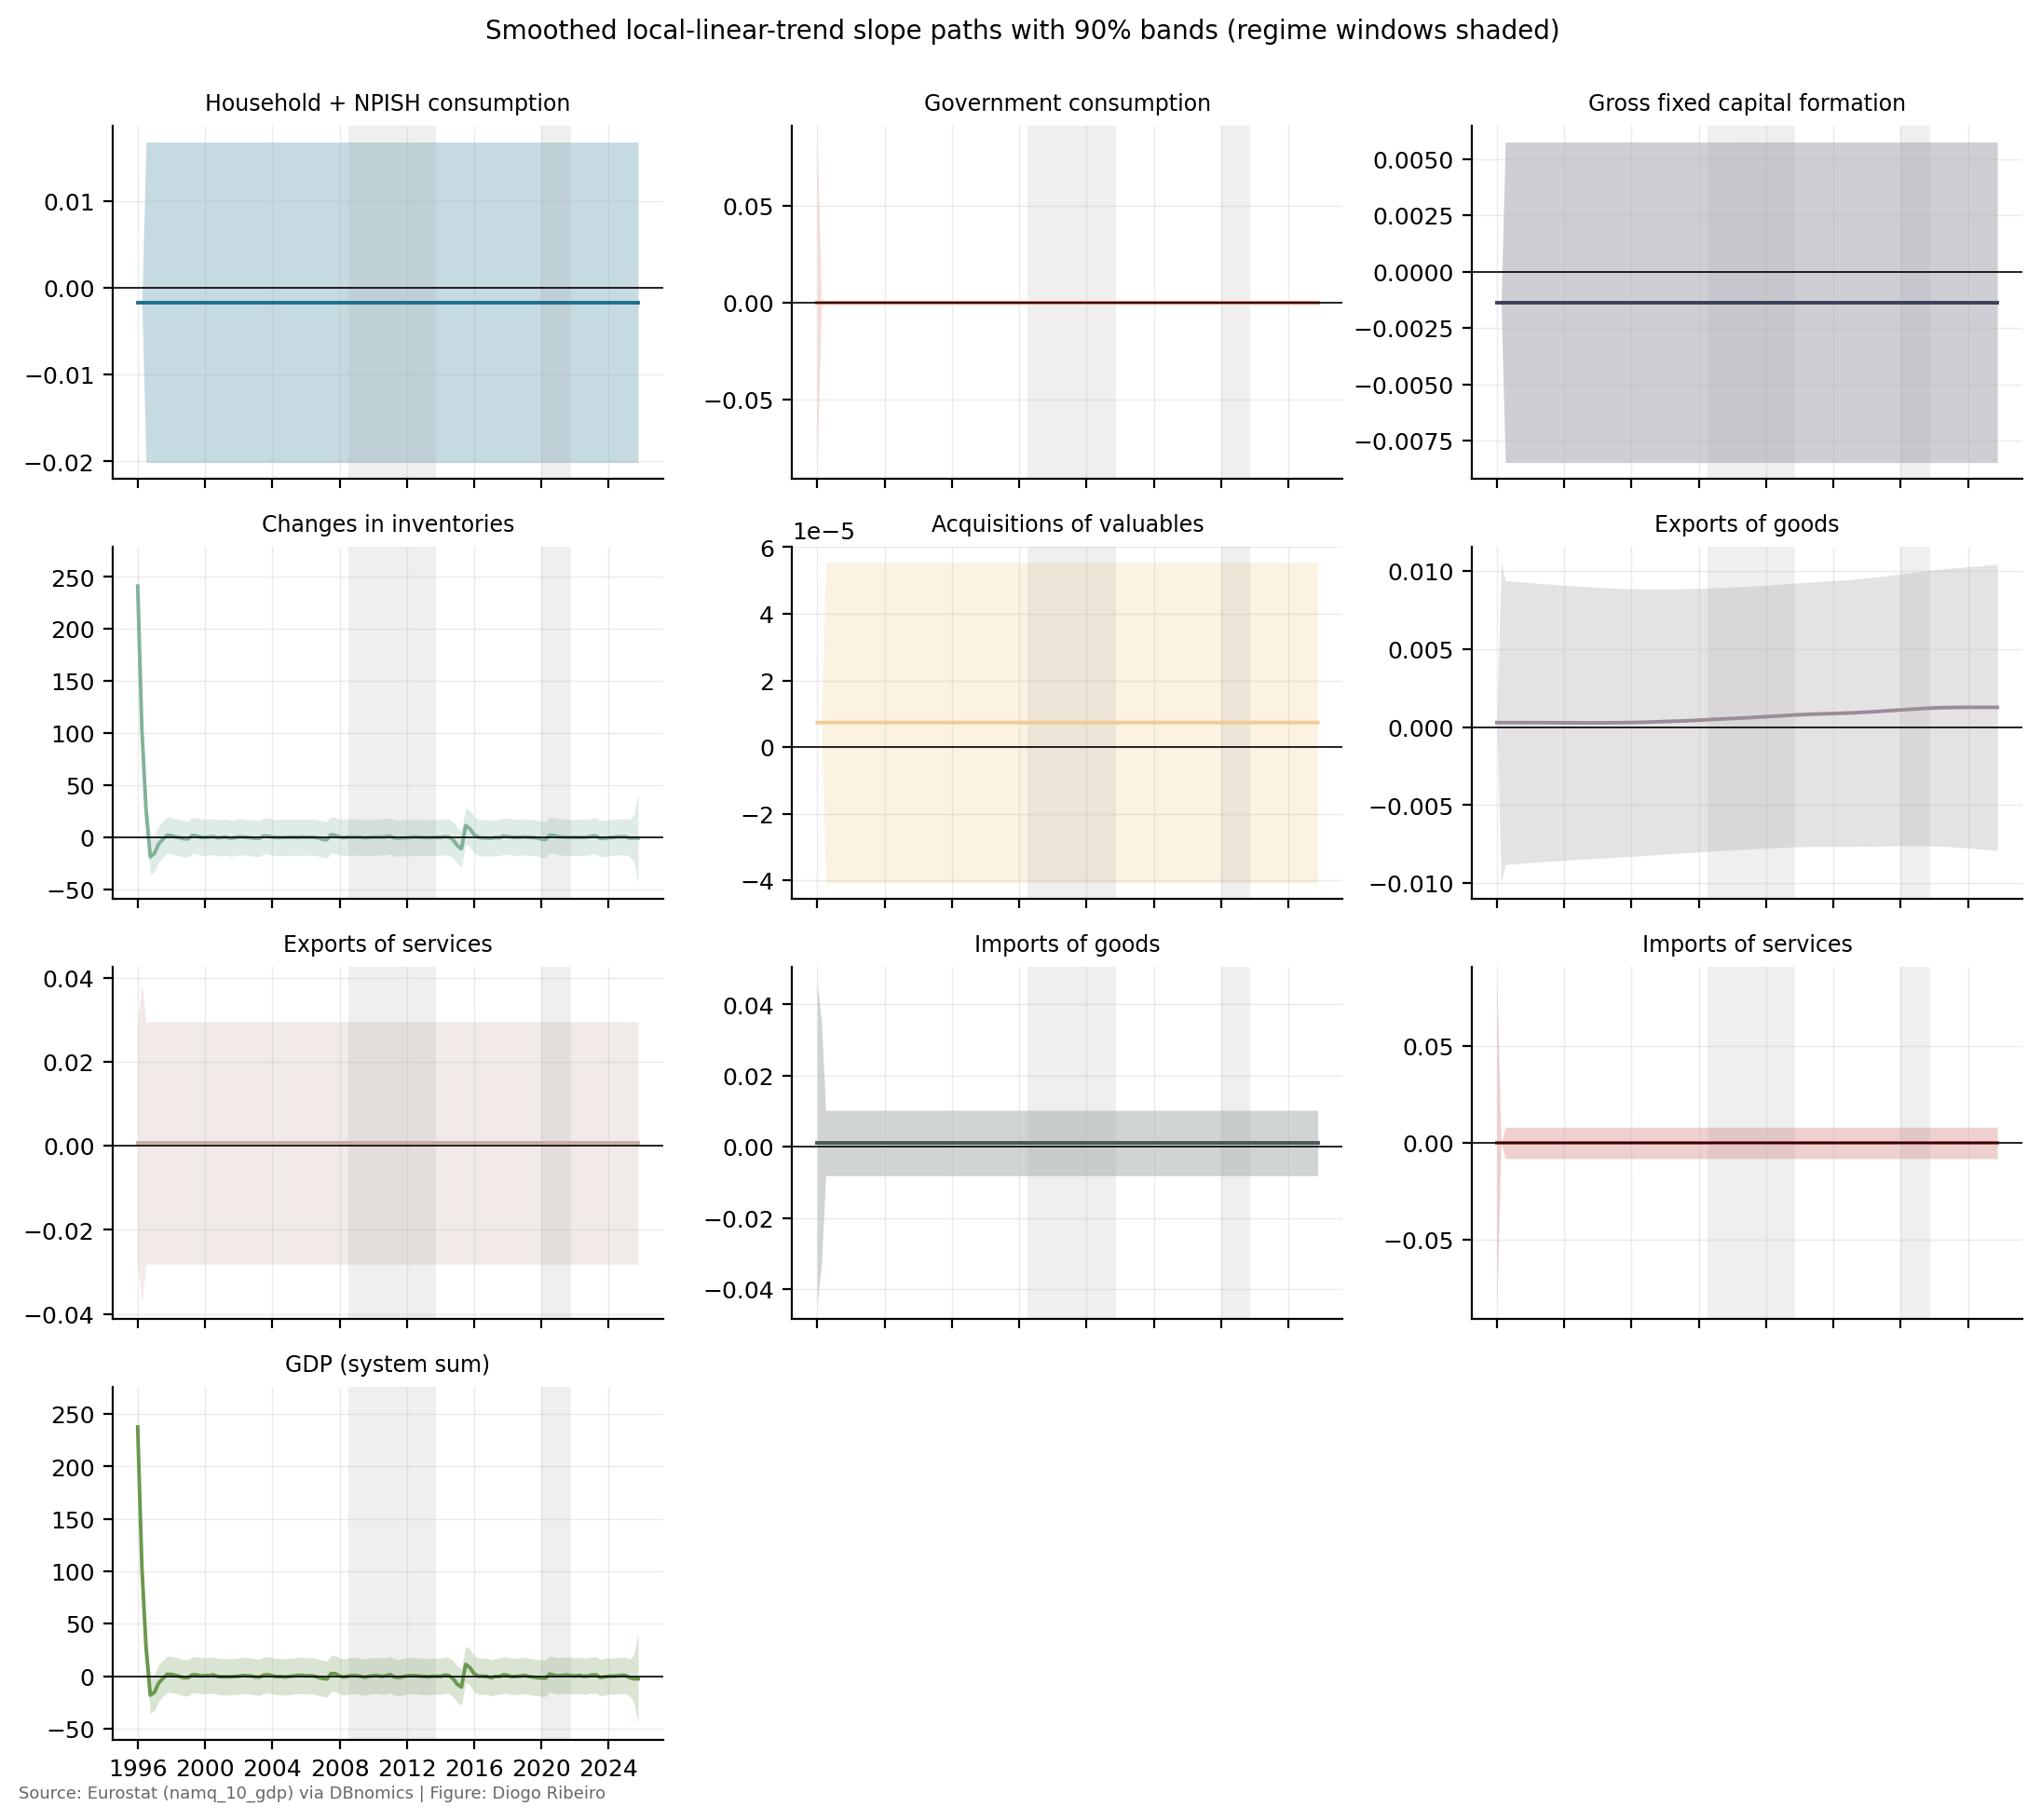
\includegraphics[width=\linewidth]{../output/slope_paths.png}
\caption{Smoothed local-linear-trend slope paths with 90\% bands}
\end{figure}


The VECM takes the long-run view, working on the log chain-linked-volume levels of the 7 strictly positive final-demand components --- inventories and valuables are excluded because they take non-positive values and their log is undefined, an exclusion that is logged rather than hidden. The Johansen trace test \cite{johansen1991} selects a cointegrating rank of 2 at the 5\% level, but with this many log-level series and only about 120 quarters the test is badly size-distorted and over-selects, so the rank is treated as descriptive and the loadings are reported for ranks 1, 2, 3 as sensitivity. The largest adjustment loading at the selected rank is on P62 (alpha = -1.230), the component that moves most to correct a departure from the long-run configuration.
\begin{figure}[H]\centering
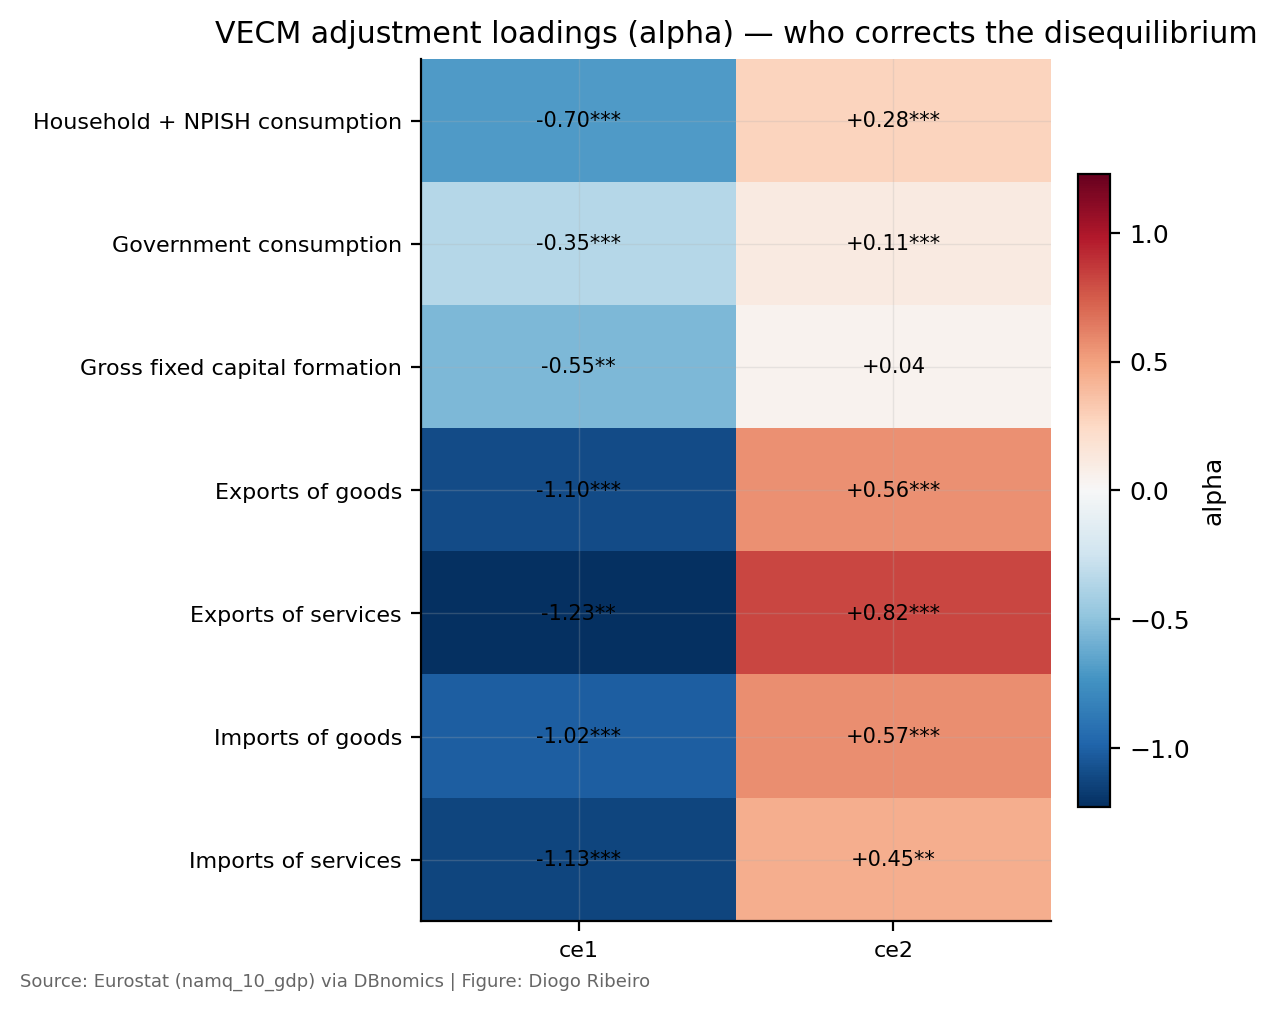
\includegraphics[width=\linewidth]{../output/vecm_alpha_heatmap.png}
\caption{VECM adjustment loadings (alpha) with significance stars}
\end{figure}


The backtest closes the dynamics section with a specification check rather than a forecasting claim: expanding-window, one-quarter-ahead forecasts of GDP growth from 2010Q1, with no look-ahead, under the SUR mean model, a sum of per-component AR(1) forecasts, and a direct AR(1) benchmark. Excluding the pandemic quarters, the SUR mean model posts an RMSE of 0.735 pp against the benchmark's 0.652 pp; over the full window the SUR RMSE is 5.967 pp. The Diebold-Mariano test \cite{dm1995} of the SUR model against the AR(1) benchmark gives a statistic of 1.363 (p = 0.173), and the summed-AR(1) decomposition a statistic of 1.049 (p = 0.294). A positive statistic means the model loses to the benchmark; where the difference is not significant, the honest conclusion is that the decomposition earns its keep as an accounting and inference device, not as a predictor that beats a one-line univariate model out of sample.
Read as a sequence, the dynamics tell one story. The diagnostics say the static mean model leaves autocorrelation on the table; the state-space slopes show that the underlying drift is genuinely time-varying and pin down the windows in which it is distinguishable from zero; the VECM asks whether the components share a long-run resting configuration and which of them does the correcting; and the backtest disciplines the whole exercise by asking whether any of this structure improves an out-of-sample forecast of headline growth. The four layers answer different questions --- completeness, timing, long-run structure, and predictive content --- and they are deliberately not collapsed into a single number, because each carries its own caveats and each would fail differently.
\section{Limitations and what would change the conclusions}
Several choices bound what can be claimed. The chain-linking residual is handled by an exact annual-overlap method with a proportional reallocation of the small remainder; a different reallocation convention would move individual contributions at the second decimal, which is why both conventions are reported side by side. The import-content adjustment is a gross-versus-net reattribution driven entirely by an exogenous input-output matrix; a different vintage would change the domestic-versus-external split, and no claim here survives replacing the placeholder shares with implausible ones. The Johansen rank selection is size-distorted at this sample length and is reported as descriptive with rank sensitivity rather than as a tested number. The state-space slopes are estimated per series, so the adding-up identity that the SUR layer guarantees is broken across the state-space models by design, and the reported per-quarter gap is the honest measure of that break. Finally, nothing in this report is a causal claim: the regime dummies and trends describe conditional means with HAC-valid standard errors, the word 'significant' is used only where a named test supports it, and the backtest is a specification check, not a forecast people should trade on.
It is worth being concrete about what would overturn, rather than merely nudge, the headline readings. The cyclical regime story --- a deep contraction across the crisis-and-troika window and a sharper, shorter pandemic swing --- is robust to the contribution convention, because it lives in the regime means of GDP growth itself, which no reallocation touches. The trend reading is the more fragile one: a small, imprecisely estimated GDP trend could change sign under a different sample window or a different treatment of the pandemic quarters, which is exactly why the state-space slope path, with its explicit bands, is the honest companion to the single trend coefficient. The long-run VECM loadings are the most tentative objects in the report and should be read as a description of which components historically absorbed disequilibria, not as a structural adjustment mechanism to be relied on out of sample. None of these caveats is a reason to withhold the decomposition; they are the terms on which it should be read.

\begin{thebibliography}{99}
\bibitem{eurostatqna} Eurostat (2013). \emph{Handbook on Quarterly National Accounts}. Publications Office of the European Union, Luxembourg.
\bibitem{kruskal1968} Kruskal, W. (1968). When are Gauss-Markov and least squares estimators identical? A coordinate-free approach. \emph{The Annals of Mathematical Statistics} 39(1), 70--75.
\bibitem{neweywest1987} Newey, W. K. and West, K. D. (1987). A simple, positive semi-definite, heteroskedasticity and autocorrelation consistent covariance matrix. \emph{Econometrica} 55(3), 703--708.
\bibitem{ljungbox1978} Ljung, G. M. and Box, G. E. P. (1978). On a measure of lack of fit in time series models. \emph{Biometrika} 65(2), 297--303.
\bibitem{engle1982} Engle, R. F. (1982). Autoregressive conditional heteroscedasticity with estimates of the variance of United Kingdom inflation. \emph{Econometrica} 50(4), 987--1007.
\bibitem{plobergerkramer1992} Ploberger, W. and Kr\"amer, W. (1992). The CUSUM test with OLS residuals. \emph{Econometrica} 60(2), 271--285.
\bibitem{harvey1989} Harvey, A. C. (1989). \emph{Forecasting, Structural Time Series Models and the Kalman Filter}. Cambridge University Press, Cambridge.
\bibitem{johansen1991} Johansen, S. (1991). Estimation and hypothesis testing of cointegration vectors in Gaussian vector autoregressive models. \emph{Econometrica} 59(6), 1551--1580.
\bibitem{dm1995} Diebold, F. X. and Mariano, R. S. (1995). Comparing predictive accuracy. \emph{Journal of Business \& Economic Statistics} 13(3), 253--263.
\bibitem{bdp2016} Banco de Portugal (2016). The import content of global demand in Portugal. \emph{Economic Studies}, Vol. II, No. 2.
\bibitem{statsmodels} Seabold, S. and Perktold, J. (2010). statsmodels: econometric and statistical modeling with Python. In \emph{Proceedings of the 9th Python in Science Conference}, 92--96.
\end{thebibliography}
\end{document}
